\section{Results}
In our experiments, we have used whole genome sequencing data of two mother-father-child trios I1 (Table \ref{tab:I1}), and G1, publish by \cite{kitzman2012}. In our experiments we have mainly used the first trio I1 with 13\% fetal admixture in obtained plasma. First, we have genotyped both the parents using Samtools and Bcftools. Subsequently we have phased the haplotypes using Beagle 4 \cite{browning2013} with reference haplotype panels from 1000 genome project.

\begin{table}[t]
\centering
\begin{tabular}{l|l|c}
Individual & Sample & DOC \\ \hline
Mother (I1-M) & Plasma (5 ml, gestational age 18.5 weeks) & 78 \\
	& Whole blood ($<1$ ml) & 32 \\
Father (I1-P) & Saliva & 39 \\
Child (I1-C) & Cord blood at delivery & 40
\end{tabular}
\vspace{3pt}
\caption{Summary of mother-father-child trio I1 sequencing data, curtsey of \cite{kitzman2012}  }
\label{tab:I1} 
\end{table}

We have simulated 360 CNVs in I1 plasma to test recall of our method, while G1 plasma sample served as a reference in DOC-based CNV estimation described in \ref{ss:coverage}. For each test case, we have picked a random position in chromosome 1, outside known centromere and telomeres region, to place the simulated CNV. Then we run our algorithm on a sequence window starting 20Mb before the simulated CNV and ending 20Mb after the CNV. If there was not enough base pairs for the beginning or end of the window, we extended the end or beginning, respectively, to get a window with 40Mb unaffected positions. We describe our simulation methods in detail in the Section \ref{ss:simulation}. The results are show in Table \ref{tab:resff13}

To test precision of our method, we run our model on the whole genome and compared our CNV calls with results of CNVnator \cite{abyzov2011cnvnator} run on pure maternal sample and child's sample obtained after the delivery.
\todo[inline]{evaluation of our calls}

\begin{table}[t]
\centering
\missingfigure{13\% results}
\begin{tabular}{l|l|c}
\end{tabular}
\caption{Summary of results for 13\% fetal admixture in plasma. }
\label{tab:resff13} 
\end{table}

Lastly, we have repeated previously described experiments on maternal plasma with down-rated fetal admixture from $13\%$ to $10\%$ and $7\%$.

\todo[inline]{DOC variance: maternal vs plasma sequencing}

\begin{figure}[h]
\center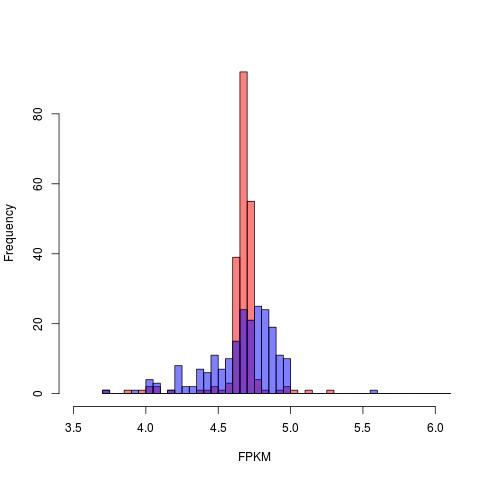
\includegraphics[width = 0.7\textwidth]{figures/fpkm}
\caption{TEXT}\label{fig:fpkm}
\end{figure}


\input simulation


